\documentclass[9pt,twocolumn,twoside]{pnas-new}
% Use the lineno option to display guide line numbers if required.
% Note that the use of elements such as single-column equations
% may affect the guide line number alignment. 

\usepackage{linguex}

\templatetype{pnasresearcharticle} % Choose template 
% {pnasresearcharticle} = Template for a two-column research article
% {pnasmathematics} = Template for a one-column mathematics article
% {pnasinvited} = Template for a PNAS invited submission

\title{Morality constrains the default representation of what is possible}

% Use letters for affiliations, numbers to show equal authorship (if applicable) and to indicate the corresponding author
\author[a,1]{Jonathan Phillips}
\author[a]{Fiery Cushman} 

\affil[a]{Harvard University, Department of Psychology, William James Hall, 33 Kirkland Street, Cambridge, MA 02138}

% Please give the surname of the lead author for the running footer
\leadauthor{Phillips} 

% Please add here a significance statement to explain the relevance of your work
\significancestatement{As humans, we think not only about what is, but also what could be. These representations of alternative possibilities support many important cognitive functions, such as predicting others' future actions, assigning responsibility for past events, and making moral judgments. We perform many of these tasks quickly and effortlessly, which suggests access to an implicit, default assumption about what is possible. What are the default features of the possibilities that we consider?  Remarkably, we find a default bias towards representing immoral or irrational actions as being impossible.  Although this bias is diminished upon deliberative reflection, it is the default judgments that appear to support higher-level cognition.} %% 117 words atm

% Please include corresponding author, author contribution and author declaration information
\authorcontributions{JP and FC conceived of and designed the studies together. JP conducted the studies and analyzed the data with input from FC. JP drafted an initial version of the manuscript, which was then revised jointly.}
\authordeclaration{The authors declare that they have no conflicts of interest.}
\correspondingauthor{\textsuperscript{1}To whom correspondence should be addressed. E-mail: phillips01@g.harvard.edu}

\keywords{Modality $|$ High-level Cognition $|$ Morality $|$ Norms $|$ Possibility}

\begin{abstract}
The capacity for representing and reasoning over sets of possibilities, or modal cognition, supports diverse kinds of high-level judgments: causal reasoning, moral judgment, language comprehension, and more. Prior research on modal cognition asks how humans explicitly and deliberatively reason about what is possible but has not investigated whether or how people have a default, implicit representation of which events are possible. We present three studies that characterize the role of implicit representations of possibility in cognition. Collectively, these studies differentiate explicit reasoning about possibilities from default implicit representations, demonstrate that human adults often default to treating immoral and irrational events as impossible, and provide a case study of high-level cognitive judgments relying on default implicit representations of possibility rather than explicit deliberation. 
\end{abstract}

\dates{This manuscript was compiled on \today}
\doi{\url{www.pnas.org/cgi/doi/10.1073/pnas.XXXXXXXXXX}}

\begin{document}

% Optional adjustment to line up main text (after abstract) of first page with line numbers, when using both lineno and twocolumn options.
% You should only change this length when you've finalised the article contents.
\verticaladjustment{-2pt}

\maketitle
\thispagestyle{firststyle}
\ifthenelse{\boolean{shortarticle}}{\ifthenelse{\boolean{singlecolumn}}{\abscontentformatted}{\abscontent}}{}

% If your first paragraph (i.e. with the \dropcap) contains a list environment (quote, quotation, theorem, definition, enumerate, itemize...), the line after the list may have some extra indentation. If this is the case, add \parshape=0 to the end of the list environment.
\dropcap{H}uman thought often involves alternative possibilities: how things could have been, might be now, or may turn out. In other words, it involves \emph{modal} cognition, a capacity to construct and reason over sets of non-actual events. Past research demonstrates a role for modal cognition in assessing causal responsibility \citep{lewis2013counterfactuals,pearl2009causality,gerstenberg2016theories}, making moral judgments \citep{kane2011oxford,hart1985causation,lagnado2013causal}, inferring what others intend to communicate \citep{portner2009modality,kratzer2012modals,stalnaker2002common}, and much more \citep{phillips2015unifying}.

To date, research on modal cognition has not distinguished between implicit and explicit representations of possibility. In fact, past methods have overwhelmingly asked how we \textit{explicitly} and \textit{reflectively} represent and reason about different possibilities. We now know a great deal about how and when people engage in explicit counterfactual reasoning, or reasoning about about what else would have happened if a given alternative event had occurred (see \cite{byrne2016counterfactual} for a recent review). There is also a small but growing amount of research on how human adults deliberate and decide whether a given event is possible or impossible \cite{shtulman2013cognitive}. In addition, there is an emerging literature on the neural substrates recruited when participants are instructed to engage in episodic counterfactual reasoning or simulation of possible future events \cite{schacter2015episodic,de2015neural}.

This research has been important for building an understanding of the way that human adults explicitly represent and reason about particular possibilities. But are these same processes recruited when humans make high-level judgments that are known to involve representations of possibilities? There is reason for doubt. Causal and moral judgments, for example, are often made quickly and effortlessly, and appear early in human development \citep{hamlin2007social,buon2013non}. Thus, these judgments are unlikely to rely exclusively on explicit deliberation about, or simulation of, alternative possibilities. Moreover, deliberative judgments about possibility often provide a poor fit to the patterns of high level judgments they supposedly inform (see, e.g., \cite{mandel1996counterfactual} on the dissociation between causal judgments and explicit counterfactual reasoning).

In light of this, an intriguing possibility is that people rely on a different kind of modal representation---one that is rendered quickly, automatically, and based on a distinctive set of constraints. This could reflect a dissociable ``system'', or instead a graded contrast between default and deliberative judgments rendered by a common system.  In either event, the aim of the present study is to test for a form of non-deliberative modal cognition, identify its signature properties, and determine its influence on higher-level cognition.

Critically, two independent research programs point toward a candidate signature property of the default representation: the relevance of prescriptive norms, such as morality and rationality. Prior research on adults' deliberative reasoning about the (im)possibility of an event shows sensitivity to \textit{descriptive} norms, such as the likelihood of the event occurring (see, e.g., \citep{shtulman2013cognitive}), but not \textit{prescriptive} norms (e.g., \citep{phillips2016do,shtulman2016differentiating}). Thus, for instance, we tend to think `It isn't possible for Lewis to open the safe' when it is highly unlikely he will guess the combination (a descriptive feature).  In contrast, we tend not to think `It isn't possible for Lewis to take the money' when it is sitting right in front of him, but belongs to somebody else (a prescriptive feature).

Remarkably, however, circumstantial evidence indicates that less explicit and reflective modal representations may be sensitive to both prescriptive and descriptive norms. That is, our default assessment of Lewis's possible actions may exclude what would be wrong in the same way that it excludes what would be unlikely.

One source of evidence comes from studies of young children. While children, much like adults, say that events that violate physical laws cannot happen (e.g., eating lightning), young children also say that events that violate moral or social norms cannot happen (e.g., stealing candy) \citep{browne2004preschoolers,kalish1998reasons,kushnir2015developing,shtulman2009development,shtulman2007improbable}. Not only do they judge these kinds of immoral events are `impossible', they even say that such events would require `magic'\citep{phillips2016do,shtulman2016differentiating}.

Additionally, some contemporary models of high-level cognition in adults argue that the underlying representation of possibility must be sensitive to both descriptive and prescriptive norms. This feature has played a critical role, for example, in understanding human causal reasoning \cite{halpern2015graded,kominsky2015causal}, modality in natural language \cite{knobe2013modals}, and judgments of force and freedom \cite{young2011paradox}, among others \cite{phillips2015unifying}. These models do not, however, provide evidence for how this modal representation is computed.

In sum, this evidence suggests that there may be a non-deliberative and early-emerging form of modal cognition that incorporates information about both descriptive and prescriptive norms. According to this hypothesis, the default representation would support not just judgments of what is `possible', but diverse modal judgments concerning what `ought', `should', `might', `may' or `could' be done, and, moreover would serve as input to diverse high-level cognitive judgments. We pursue these hypotheses in three sets of studies.

\section*{Study 1: Deliberative vs. default representations of possibility}

To investigate whether there are differences in more and less deliberative forms of modal cognition, we began by focusing specifically on judgments of possibility, asking participants to make judgments of whether various events were `possible' or `impossible', while manipulating the amount of time available for this judgment. These judgments were made in the context of some background information, such as \ref{context}:

\ex. \label{context} Josh is on the way to the airport to catch a flight for a hunting safari in Africa. He leaves with plenty of time to make it there, but his car breaks down on the highway. Now Josh is sitting in his car near a busy intersection, and knows he needs to get to airport soon if he is going to catch his flight.

\noindent Participants read six different background contexts, and after each one they were shown a series of candidate events one at a time. As each event was presented, participants pressed a key to indicate whether they thought that the event was `possible' or `impossible'. Crucially, participants were either forced to make these judgments very quickly ($\leq 1500 ms$) or were asked to reflectively deliberate on the possibility of each event ($\geq 1500 ms$). We used a total of 144 different events, which were designed to fall into five categories: 48 ordinary events that did not violate any norms, e.g., \ref{ordinaryEvent}, 24 events that violated statistical norms, e.g., \ref{improbableEvent}, 24 events that violated physical laws, e.g., \ref{impossibleEvent}, 24 events that violated moral rules, e.g., \ref{immoralEvent}, and 24 events that violated norms of rationality, e.g., \ref{irrationalEvent}. (The a priori categorization of these events were confirmed in independent ratings of the morality, probability, and rationality of each of the events, see \textit{SI: Event Ratings}.)

\ex.  Is it possible or impossible for Josh to...
\a. \label{ordinaryEvent} hail a taxi at the intersection.
\b. \label{improbableEvent} fix his car by banging on it.
\c. \label{impossibleEvent} teleport himself to the airport.
\d. \label{immoralEvent} sneak onto public transportation.
\e. \label{irrationalEvent} sell car for ride to airport.

This paradigm uses judgments of whether an event is `possible' as an indicator of whether participants represent that event as being available in the context. By changing the amount of time participants have to deliberate, we ask whether (and how) participants' representation of the set of available events changes as a result of more or less deliberation.

\subsection{Results} We first used a series of linear mixed-effects models to test whether participants' judgments of the possibility of the five different kinds of events differed across time pressure/delay conditions (see \textit{SI: Statistical Approach}). We observed an effect of whether participants were reflectively deliberating, $\chi^2(1) = 20.653$, $p < .001$, and an effect of event-type  $\chi^2(4) = 860.48$, $p < .001$. Critically, however, these main effects were qualified by a deliberation*event-type interaction, $\chi^2(4) = 64.093$, $p < .001$. We decomposed this interaction using a series of generalized linear models. These revealed that deliberation did not significantly affect participants' judgments of the possibility of \textit{ordinary} events ($z = -0.164$, $p = 0.87$), or \textit{improbable} events ($z = -1.056$, $p = 0.291$). While not predicted, participants more tended to judge that events that violated physics were impossible after deliberating ($M = 85.22$, $SD = 17.44$), than when forced to answer quickly ($M = 79.37$, $SD = 15.82$), ($z = -6.628$, $p < .001$). Critically, however, we found that participants' judgments of the possibility of immoral and irrational events was affected by deliberation in the opposite direction. They tended to judge that immoral events were impossible when they were not able to reflectively deliberate ($M = 37.30$, $SD = 30.21$), but more judged them to be possible after deliberating ($M = 21.41$, $SD = 31.26$), ($z = 5.423$, $p < .001$). Similarly, they  tended to judge that irrational events were impossible more when they were not able to deliberate ($M = 42.10$, $SD = 25.89$), than after deliberating ($M = 37.86$, $SD = 30.89$), ($z = 1.963$, $p < .05$) (see \textbf{Fig.} \ref{fig:fig1}).

In short, we find evidence that default representations of what is possible differ from more reflective representations in that prescriptive norms selectively constrain the default representation of possibility. Moreover, two key contrasts support a role for moral norms in particular: judgments of the possibility of immoral events were more affected by deliberation than either improbable events $\chi^2(1) = 28.035$, $p < .001$, or irrational events $\chi^2(1) = 24.937$, $p < .001$, despite the fact that all of these events involved clear norm violations.

\begin{figure}%[tbhp]
\centering
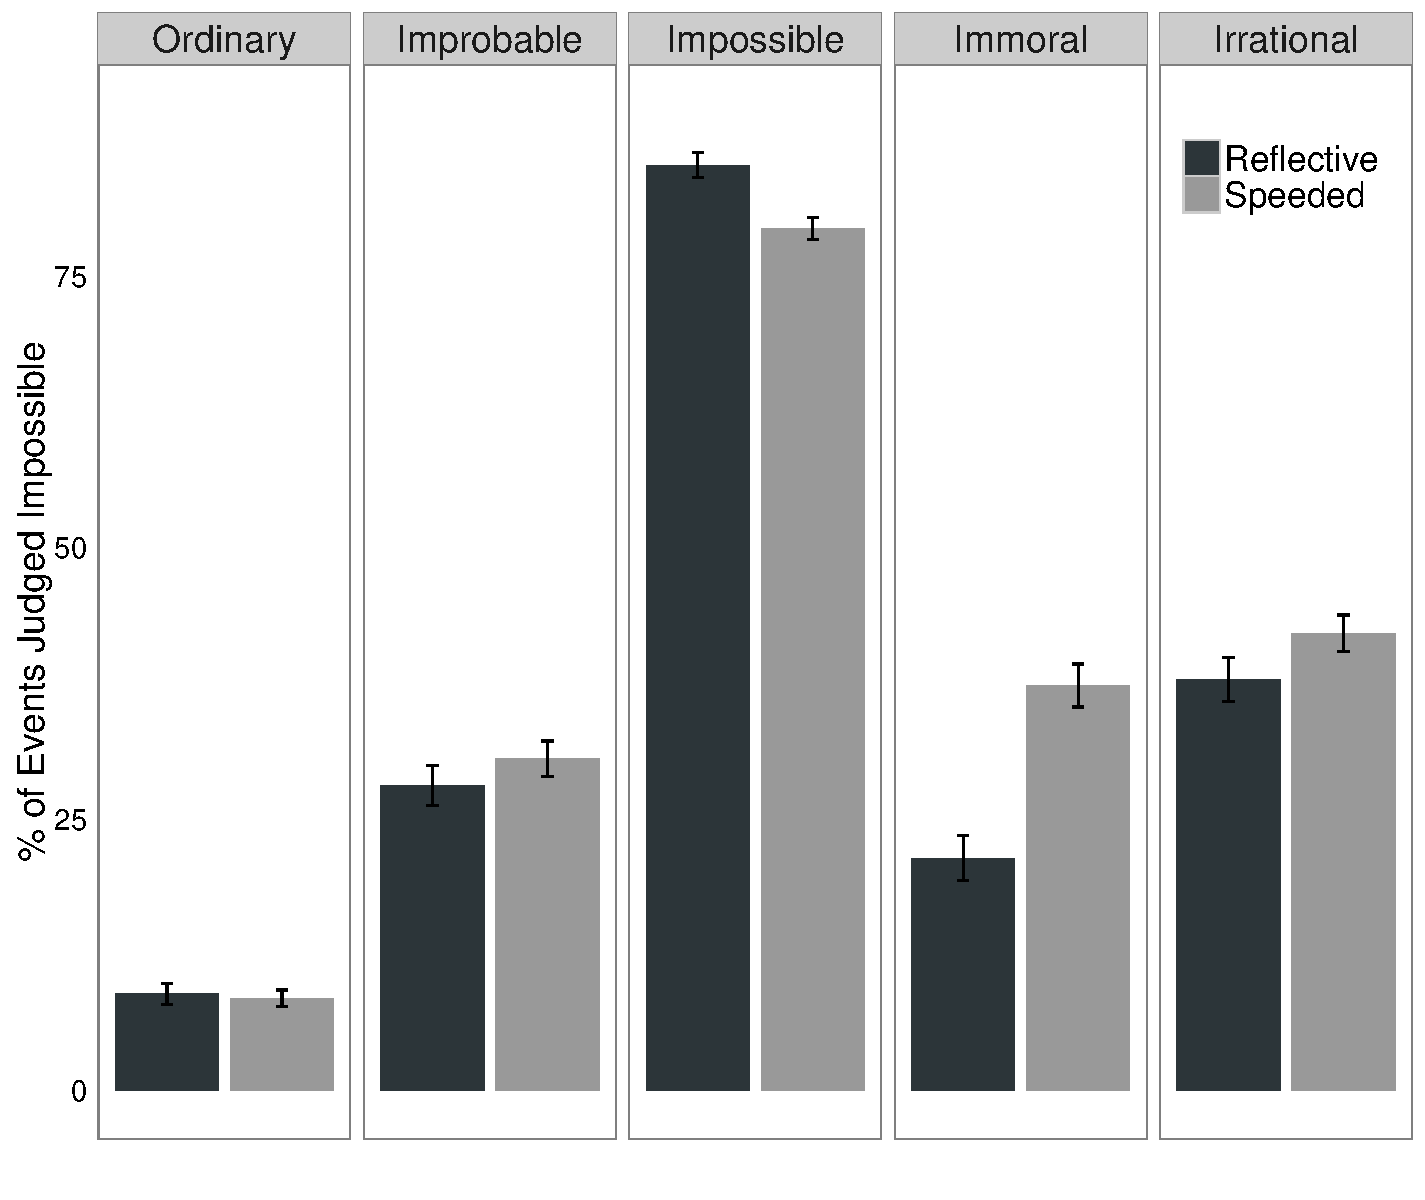
\includegraphics[width=.9\linewidth]{fig1}
\caption{Judgments of impossibility for five different kinds of events when participants made judgments after deliberating (dark bars) or without time to deliberate before responding (light bars). Error bars indicate +/- 1 SEM.}
\label{fig:fig1}
\end{figure}

\section*{Study 2: Does this default generalize across modal judgments?}

All modal judgments involve reasoning over sets of possibilities. Linguistically, however, different modal auxiliaries (e.g., `might' vs. `ought') are known to select different sets of possibilities \citep{portner2009modality,kratzer2012modals}. This distinction is also reflected in non-linguistic cognition: we think differently about what a person `could' or `might' do than we do about what they `should' or `ought' to do. In all of these cases though, these judgments require us to reason over the set of events that are represented as being available in the context. Accordingly, we can ask if the observed differences across different kinds of modal auxiliaries are essential to the default representation of each different modal, or if they are instead the result of additional processing required to move away from a single, unified default representation of possibility.

We propose that there is a common mechanism responsible for rapidly constructing a default representation of what is possible, which supports diverse cognitive functions. This proposal predicts that any deviation from the default representation will require additional processing, and thus the selection of \textit{different} sets of possibilities for different modal judgments is likely the result of more deliberative cognition. This prediction is testable: we can ask whether the correlation between judgments of what a person `could' do, `might' do, `ought' to do, etc. is higher when people do not have time to reflect (and thus more rely on a default representation of possibility), and lower when people do have time to reflect before making a modal judgment.

An obvious alternative prediction is that reducing the amount of time that participants have to respond should increase the noise observed in their responses. This predicts that modal judgments will instead be less correlated with one another when they have to be made extremely quickly (compared to when they are made with time to reflect). We hypothesized that this effect would be outweighed by the influence of a common default modal representation.

Motivated by the results of Experiment 1, we further hypothesized that the default representation underlying diverse modal judgments would be sensitive to prescriptive norm violations. In other words, we hypothesized that under time pressure participants' judgments of what a person could do, may do, might do, etc. would be sensitive to whether that action is immoral or irrational.  This common sensitivity to prescriptive norms should thus be largely responsible for heightened similarity among the default representations elicited by diverse modals.

Following the basic procedure introduced Experiment 1, we collected deliberative vs. non-deliberative judgments of what agents `may' do (Study 2a), `might' do (Study 2b),`could' do (Study 2c), `ought' to do (Study 2d), or `should' do (Study 2e). We also included judgments of what it is `possible' for them to do (from Study 1). These different modal terms are known to express different kinds of modality (metaphysical, circumstantial, deontic), and the overall patterns of responses demonstrate that participants tracked these differences (see \textit{SI: Differences across modal auxiliaries})

\subsection*{Results} Our analyses treat the 144 different events as the primary unit of analysis. For each of the six modal judgments, we calculated the proportion of the time that the modal judgment was accepted vs. rejected for each event, doing so independently for trials when participants had time to reflect and when they did not. These scores reflect the likelihood that an event will be included in the set of possibilities relevant to each type of modal concept (e.g., what should be done, what could be done, and so on). We then calculated the correlation between the events' representations for each possible pair of different modal judgments, both when participants were given time to reflect before answering and when they were not.

  As hypothesized, modal judgments were significantly more correlated when participants did not have time to reflect ($M_{r} = 0.893$, $SD_{r} = 0.060$) than when they did ($M_{r} = 0.830$, $SD_{r} = 0.101$), $t(14) = 5.131$, $p  < .001$, $d = 0.754$ (see Fig. \ref{fig:fig2}). This finding supports the view that participants relied on a common default representation of the set of available events when answering quickly. By contrast, when participants reflected on each judgment, their responses were more strongly dictated by unique features of each modal concept, and thus became less correlated with one another.

\begin{figure}%[tbhp]
\centering
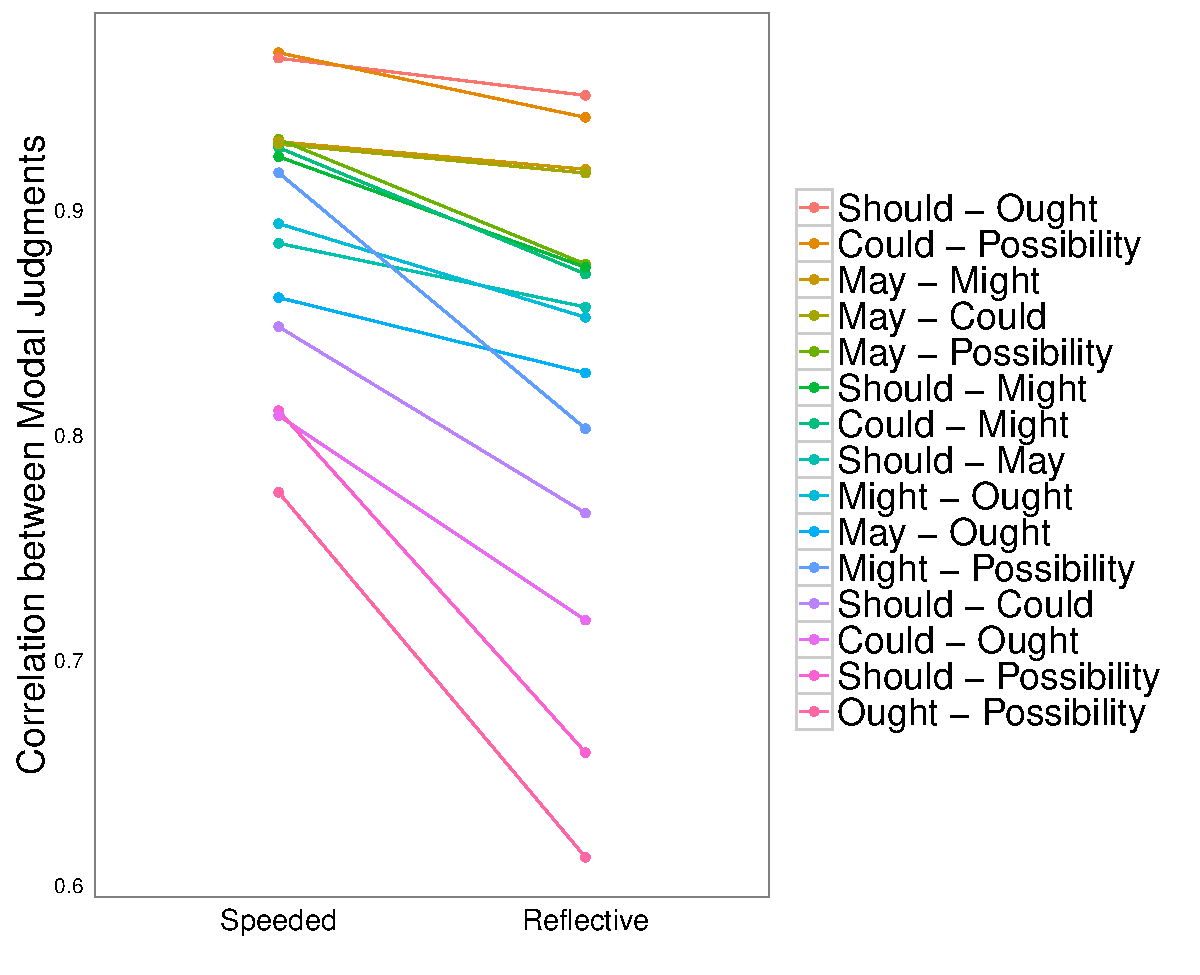
\includegraphics[width=.9\linewidth]{fig2}
\caption{Correlation coefficient of each pair of modal questions, either when participants were forced to answer quickly (left) or when they were given time to reflect before answering (right)}
\label{fig:fig2}
\end{figure}

We next asked whether a principal dimension on which default judgments became more similar was sensitivity to prescriptive norms. To do this, we divided the events that participants judged into two categories: those for which descriptive norms were primarily relevant (the improbable and physically impossible events), and those for which prescriptive norms were primarily relevant (the irrational and immoral events). We then again calculated the correlation between each pair of modal judgments, first focusing on events where descriptive norms were relevant, and then second focusing on events where prescriptive norms were relevant. This analysis allows us to ask whether it was the presence of one of these kinds of norms that was responsible for the difference in correlations when participants reflected before answering.

Analyzing these correlations with linear mixed effects models, we found an interaction effect between the type of norms that were relevant and whether or not participants had time to reflect, $\chi^2(1) = 24.323$, $p < .001$. Decomposing this interaction, we first focused on modal judgments made in scenarios for which descriptive norms were primarily relevant (e.g., winning the lottery). Here, we observed a modest decrease in the correlation between the modal judgments when participants reflected before answering ($M_{r} = 0.873$, $SD_{r} = 0.055$) from when they answered before reflecting ($M_{r} = 0.908$, $SD_{r} = 0.042$), $t(14) = 5.336$, $p  < .001$, $d = 0.724$. Next, we focused on judgments made in scenarios for which prescriptive norms were relevant (e.g., theft) and found a much larger decrease in the correlations between the modal judgments made when participants reflected before answering ($M_{r} = 0.278$, $SD_{r} = 0.265$), as compared to when they answered before reflecting ($M_{r} = 0.628$, $SD_{r} = 0.145$), $t(14) = 8.841$, $p  < .001$, $d = 1.642$ (see Fig. \ref{fig:fig3}). A corollary finding is that deontic modals show less of a difference between deliberative and reflective responses than metaphysical or circumstantial modals (see \textit{SI: Within-modal correlations}). 

\begin{figure}%[tbhp]
\centering
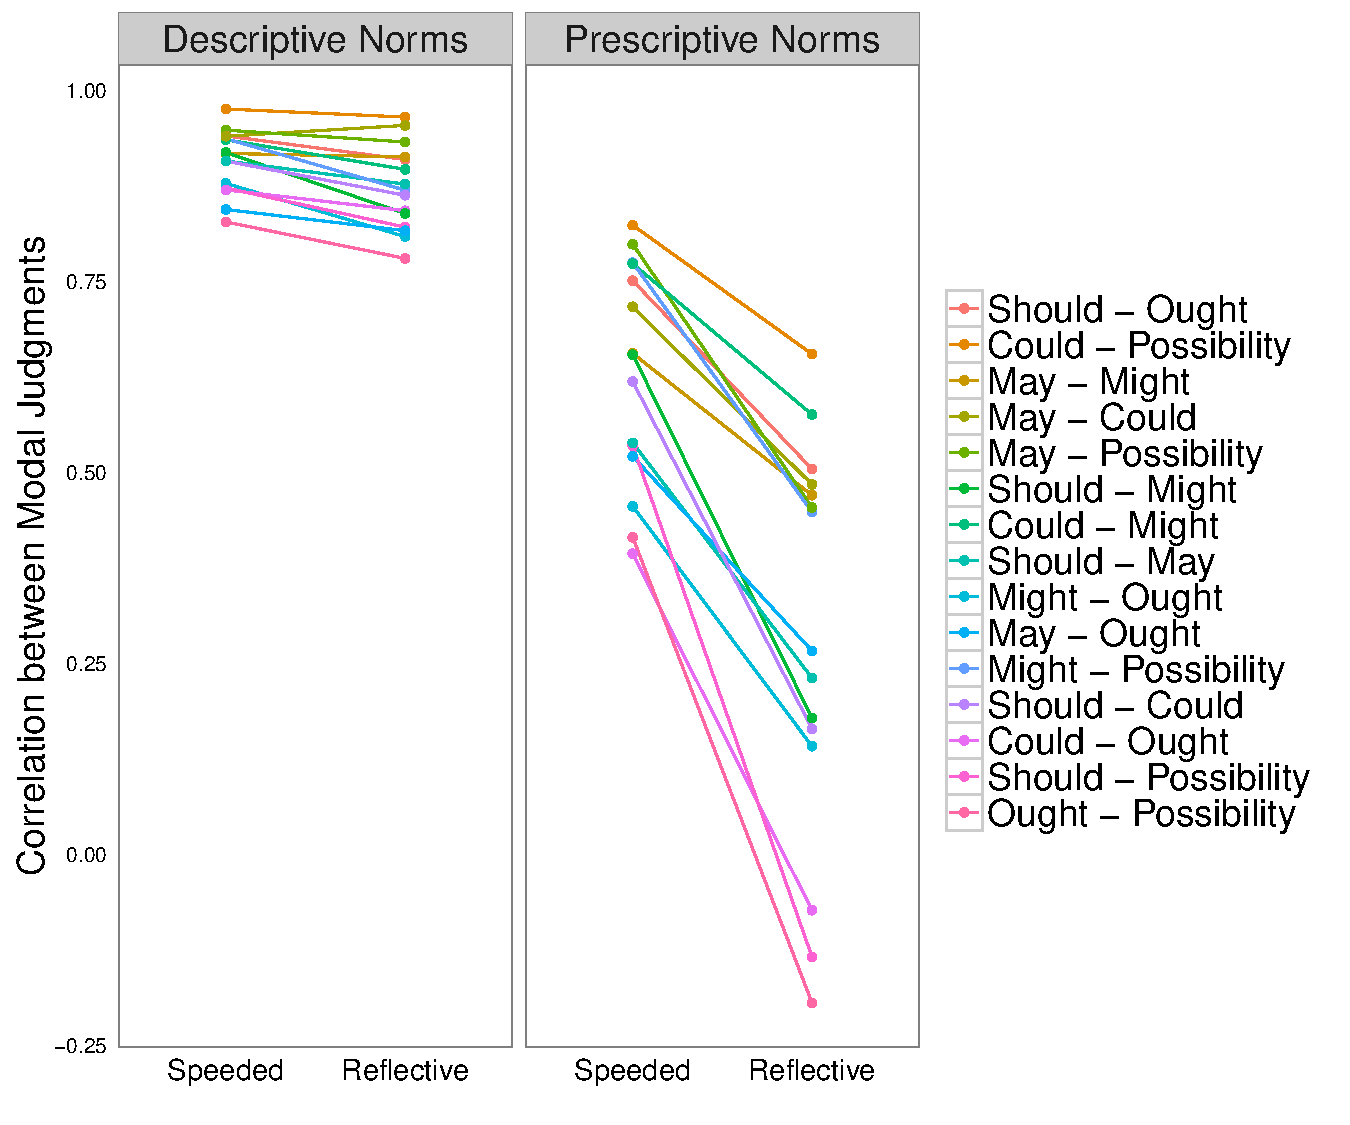
\includegraphics[width=.9\linewidth]{fig3}
\caption{Correlation coefficient for each pair of modal judgments either for items where descriptive norms were primarily relevant (left panel) or for items where prescriptive norms were primarily relevant (right panel). Correlations between modal judgments made without time to reflect are plotted on the left-hand side of the panel; correlations between modal judgments made after reflecting are plotted on the right-hand side of the panel.}
\label{fig:fig3}
\end{figure}

Together, these analyses indicate that prescriptive norms constitute a principal dimension differentiating specific modal concepts from their common default. In contrast, the use of descriptive norms appears to be relatively more consistent across distinct modal concepts, even upon reflection. This pattern is most evident for moral norms. Focusing specifically on the immoral events, which clearly distinguish different kinds of modal reasoning, we created a correlation matrix of all of the different judgments. This approach revealed that all of the different modal judgments were highly correlated when participants were not able to reflect ($0.558 \leq r \leq 0.919$), but were not when participants took time to reflect ($-0.016 \leq r \leq 0.572$) (see Fig. \ref{fig:fig4}). A corollary finding is that participants' non-reflective modal judgments are all highly correlated with \textit{reflective} judgments of what agents `ought' to do ($r_{Mean} =0.465$), but not other reflective judgments ($ -0.091 < r_{Mean} > 0.264$). Put simply, when answering quickly, modal judgments become more ought-like (see box in Fig. \ref{fig:fig4}).

\begin{figure}%[tbhp]
\centering
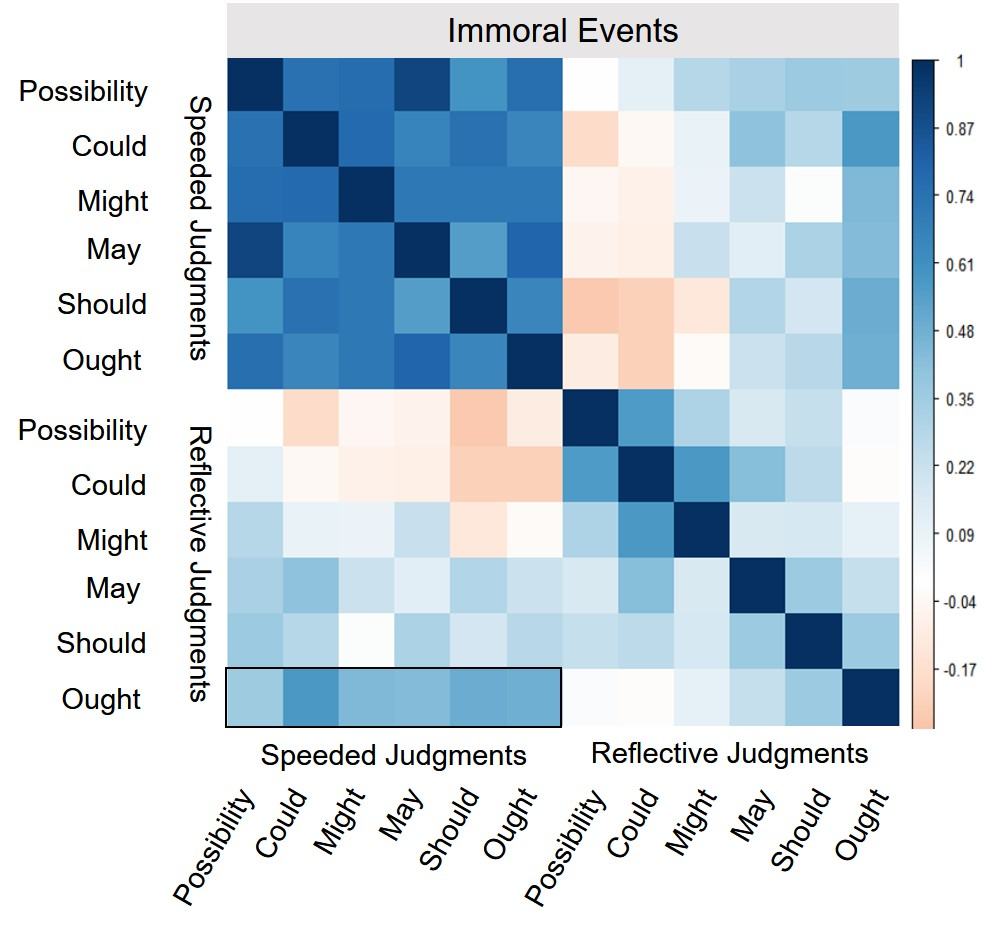
\includegraphics[width=.9\linewidth]{Fig4}
\caption{Graphical depiction of the correlation matrix for speeded and reflective modal judgments of events that involved immoral actions. Squares within the black box depict correlations of speeded modal judgments with reflective judgments of `ought'.}
\label{fig:fig4}
\end{figure}

In summary, we have demonstrated thus far that default modal judgments show a common sensitivity to both descriptive and prescriptive norms. In contrast, reflective modal judgments can deviate away from this default, allowing for some kinds of modal cognition (e.g., thoughts of what `could' happen) to focus primarily on what is physically possible, without regard to immorality or irrationality.

\section*{Study 3: Default modal representations in high-level cognition}

Existing evidence suggests that the modal representations used in other domains of high-level cognition---for instance causal attribution, language comprehension and moral judgment---are similar to the default representations identified in Experiments 1 and 2. For instance, causal judgments of an event are sensitive to the moral status of alternative events (see, e.g., \citep{Hitchcock2009,halpern2015graded}), which is consistent with the demonstrated role of prescriptive norms in default modal representations. This current evidence is indirect, however, and the role of alternative events in causal cognition remains controversial (see, eg., \citep{samland2016prescriptive}). Accordingly, Study 3 provides a direct test of the hypothesis that the default representations of the set of events available in a given context are exported to other cognitive domains.

To do this, we used judgments of `force' as a case study. This is an ideal test because empirical  \citep{phillips2009moral,young2011paradox} and theoretical \citep{berlin1970four,rowe2002nicomachean} studies concur that judgments of `force' rely on representations of alternative possibilities. Put simply, if an agent was `forced' to act in some way, this implies that there was no relevant alternative; and if she was not forced, this implies that some alternative existed. We therefore asked: when people decide whether an agent was `forced' to do something, do they rely on a set of possibilities more like a deliberative set, or instead the implicit set that we identified in Study 1?

Participants in this study once again read the six different background contexts used in the previous studies (see \ref{context}). However, in this case, the agent asked another person for advice about what to do. This person then directly suggested that the agent pursue one of the ordinary, immoral, irrational or improbable events used previously \ref{ordinaryEvent}-\ref{irrationalEvent}, as in \ref{advice}. 

\ex. \label{advice} Josh calls his father who lives a few states away and tells him about about his problem. Not really knowing how to help him, Josh's father makes a suggestion. His father says Josh could \textit{sneak onto public transportation}.

\noindent Participants were then told that, notwithstanding this advice, the agent decided to pursue some specified alternative course of action, as in \ref{decision}. 

\ex. \label{decision} Josh ignores his father’s suggestion and decides to book the next available flight, even though it is quite expensive.

Within each context, the agent was always described as pursuing the same course of action, regardless of the advice given.

After reading all of this information, participants were asked whether they agreed or disagreed that the agent was forced to do the action he or she actually pursued, as in \ref{force}.

\ex. \label{force} Josh was forced to book the next available flight.

Following previous work on judgments of force \citep{young2011paradox,rowe2002nicomachean,berlin1970four}, participants should only judge the agent to have been forced if they believe that there were not other options available to the agent---in other words, if the set of relevant alternative possibilities was empty. Thus, in the context of the specific advice given to the agent, participants should only agree that the agent was forced if they did not represent the proposed option as an available possibility.

Crucially, in all cases, the judgments of force were made with unlimited time available. Thus, our question is whether \textit{deliberative} judgments of force for each scenario are better predicted by deliberative or speeded judgments of possibility for the same scenario in Study 1.  We hypothesized that force judgments would be best predicted by speeded possibility judgments, reflecting a dominant influence of the default representation of the set of available events.

\subsection*{Results} We computed the average agreement that the agent was forced to do a given action when the alternative proposed was one of the events used in the previous studies. We then first asked whether participants' non-reflective judgments were predictive of judgments of force in a simple linear model, and found that they were, $F(1,118)=46.12$, $p<.001$, $\eta^2=0.281$ (see \textbf{Fig}. \ref{fig:fig5}). Next, we asked whether reflective or non-reflective judgments of possibility were a better predictor of judgments of force by comparing a series of linear mixed-effects models. We found that including reflective judgments of possibility did not significantly improve a model that already included non-reflective judgments of possibility, $\chi^2(1) = 0.030$, $p = .863$. In contrast, including non-reflective judgments of possibility did significantly improve a model that already included reflective judgments of possibility $\chi^2(1) = 27.640$, $p < .001$. Thus, above and beyond reflective judgments of what is possible, the default representation of possibility is predictive of deliberative judgments of force.

We next asked whether morality had an effect on judgments of force (as found in previous work \citep{young2011paradox,phillips2009moral}) and whether this effect was mediated by non-reflective judgments of possibility. We found that this was the case: participants judged agents to be more forced when the proposed alternative was immoral vs. ordinary, $t(70) = 7.309$, $p < .001$, $d = 1.827$. Moreover, this effect was mediated by non-reflective judgments of possibility, 95\%CI [0.018,0.542], $p = 0.04$. A similar pattern of results was also observed for events that involved violations of rational norms ($t(70) = 5.462$, $p < .001$, $d = 1.366$; 95\%CI [0.045,0.864], $p = 0.04$). These results fit well with ongoing work that offers a semantics for `force' according to which prescriptive norms impact the set of actions available to an agent \cite{mandlekern2017force}. (See \textit{SI: Study 3b} for a test of an alternative semantics for `force' that proposes to account for the impact of norms through inferences about the agents' desires.)

\begin{figure}%[tbhp]
\centering
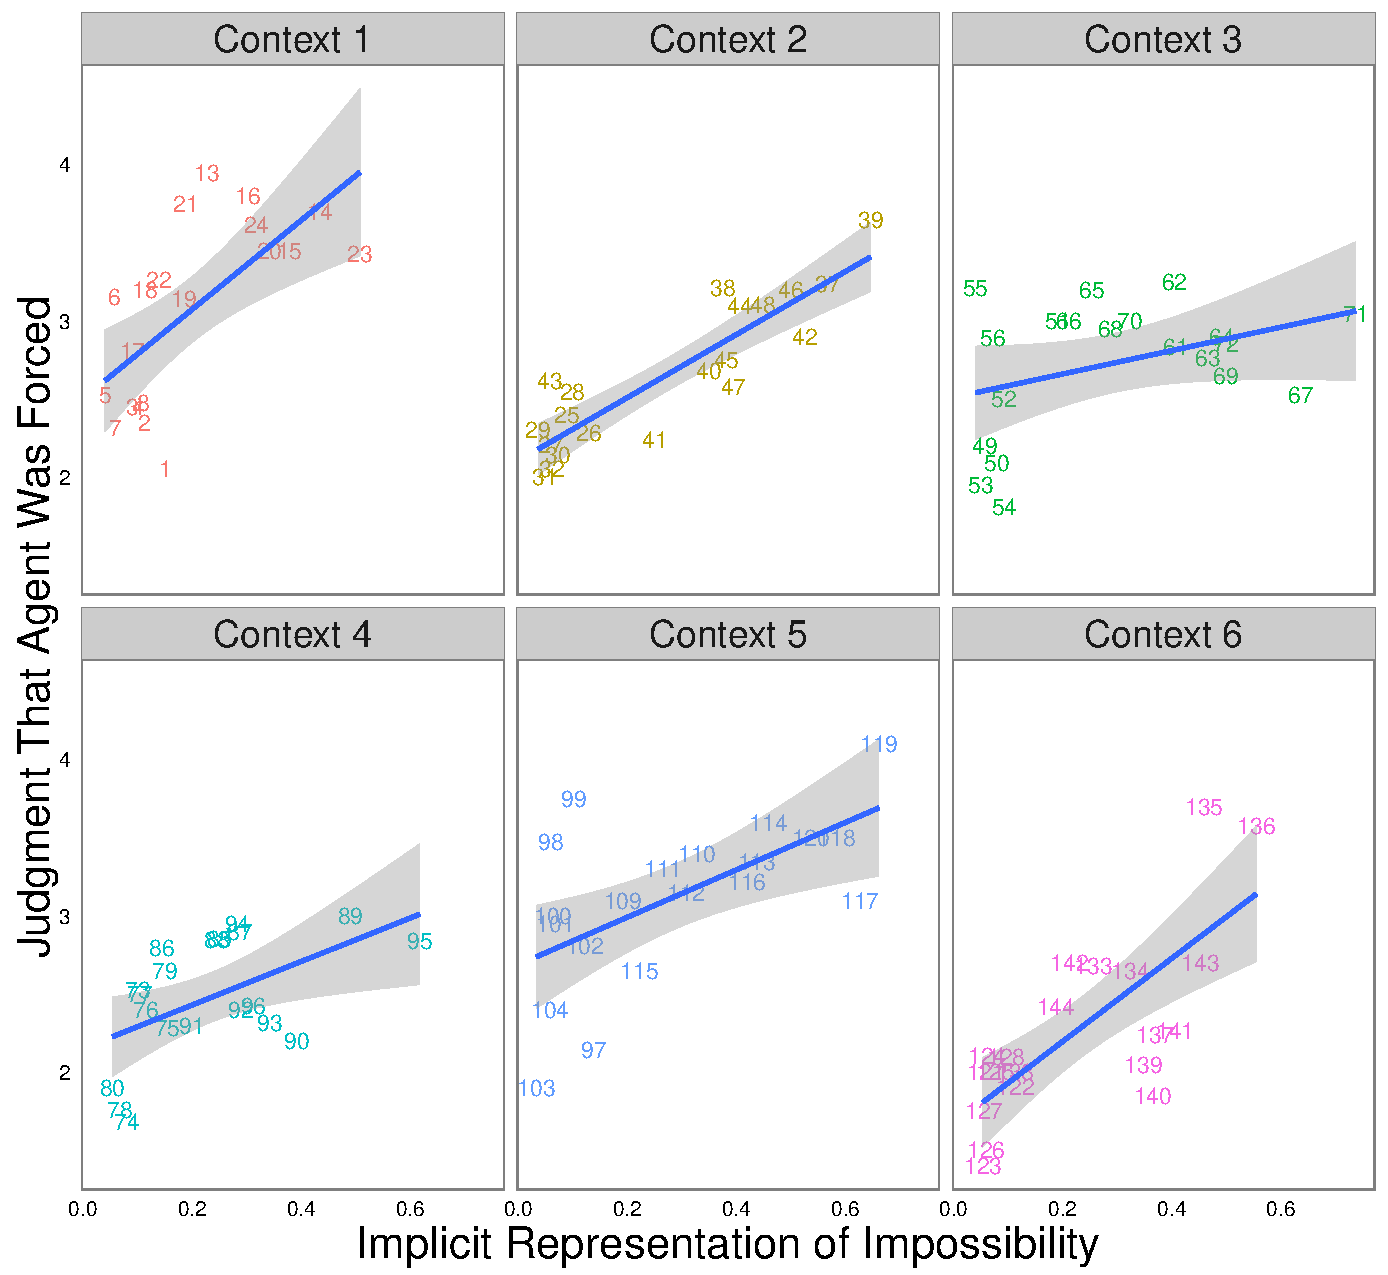
\includegraphics[width=.9\linewidth]{fig5}
\caption{Relationship between the implicit representation of possibility and high-level judgments of whether or not an agent was forced to do a given action in six different contexts. Shaded areas represent 95\% confidence intervals.}
\label{fig:fig5}
\end{figure}

\section*{Discussion}

We find evidence for a default representation of what is ``possible''--i.e., a set of events, specific to a context, that constitutes a starting point for understanding non-actual alternatives. Moreover, a hallmark of this default representation is that it tends to exclude immoral actions.  First, we found that time pressure makes people less likely to judge it possible to act immorally or, to a lesser extent, irrationally. Second, we found that this effect is reflected across diverse modal concepts: what a person ought to do, may do, could do, should do, or might do. These judgments appear to share a common default basis, and become more differentiated only after deliberative processing. Finally, as a case study of the role of implicit modal cognition in reflective high-level judgments, we found that default modal judgments are better predictors than reflective modal judgments of people's decisions about whether a person was `forced' to act in a particular way. A mediation analysis indicates that, to the extent that we are ``forced'' to act morally, it is because our default representation of what is possible tends to exclude immoral actions.

Although all forms of modal cognition involve constructing and reasoning over sets of possibilities, it is remarkable that they apparently begin with a common default template. By analogy, all forms of social cognition---whether about in-groups or out-groups, cooperators or competitors---involve reasoning about other people, but it would be remarkable to discover that under time pressure, all forms of social cognition begin with a representation of the very same people.  In modal cognition, much like in social cognition, one might have initially thought that even rapid categorizations of what it is `possible' for a person to do and what a person `ought' to do would depend on separate processes that pick out separate events. After all, most people would say that it is \emph{possible} to run a red light at an empty intersection, but not that you \emph{ought} to.

In contrast to this intuition, our findings suggest that it takes time to come to the conclusion that it is possible to run a red light: we begin with a default representation of possibility that tends to excludes this action, along with other immoral or irrational acts. The purpose of this default mechanism is a key area for further study. One appealing possibility is that the default representation serves the function of proposing actual candidate actions during decision-making---in other words, it helps us to construct a choice set \citep{ben1995discrete}. It is natural to suppose that screening out immoral or irrational actions from one's own decision-making would tend to be adaptive.

Importantly, the default representation we have uncovered bears a striking resemblance to the pattern of possibility judgments observed early in human development \citep{phillips2016do,shtulman2016differentiating,shtulman2007improbable,kalish1998reasons}. In both cases, judgments of possibility are sensitive not only to descriptive norms but also to prescriptive ones. The similarity of these patterns presents the intriguing possibility that the modal representation observed early in development is retained in adult cognition alongside a separate later-developing capacity for deliberatively reasoning about possibilities. Future work should continue to explore this connection directly, and ask which other factors serve to constrain both of these representations of possibilities.

Finally, it is worth noting a potential connection between our research and the widespread, surprising presence of moral norms in disparate corners of the human mind: e.g, in causal reasoning and mental state attribution \citep{Knobe2003,Hitchcock2009,halpern2015graded,kominsky2015causal,phillips2015unifying}. These processes also involve reasoning over a set of possibilities. Given the present results, an exciting possibility is that morality shapes how we think about many things because it constrain the very possibilities that come to mind.

\vspace{-0.1cm}
\matmethods{
\vspace{-0.5cm}
\subsection*{Participants} All participants were recruited from Amazon Mechanical Turk (\href{www.mturk.com}{www.mturk.com}) through TurkPrime (\href{ww.turkprime.com}{www.turkprime.com}), which was used to prevent repeat participation across the studies. Sample sizes and demographic information is as follows. Study 1a (judgments of possibility), 498 participants ($M_{age} = 33.85$, $SD_{age} = 10.82$, 233 females). Study 1b (event ratings), 61 participants ($M_{age} = 31.53$, $SD_{age} = 7.87$, 25 females). Study 2a (ought), 301 participants ($M_{age} = 33.40$, $SD_{age} = 9.87$, 147 females). Study 2b (might), 201 participants ($M_{age} = 33.79$, $SD_{age} = 10.20$, 92 females). Study 2c (could), 304 participants ($M_{age} = 34.87$, $SD_{age} = 11.32$, 144 females). Study 2d (may), 200 participants ($M_{age} = 32.80$, $SD_{age} = 9.21$, 86 females). Study 2e (should), 297 participants ($M_{age} = 34.05$, $SD_{age} = 9.86$, 153 females). Study 3 (force judgments), 400 participants ($M_{age} = 38.05$, $SD_{age} = 12.73$, 218 females). Study 3b (desire judgments), 400 participants ($M_{age} = 36.61$, $SD_{age} = 11.80$, 200 females). These studies were approved by the Harvard University Institutional Review Board, IRB14-2016, and informed consent was acquired from all participants.

\subsection*{Access to data, analysis code, and materials} All materials used to conduct these studies and analyze the results are available at: \href{github.com/phillipsjs/implicitModality}{github.com/phillipsjs/implicitModality}. Studies 1a-b and 2a-e were conducted through Testable (\href{www.testable.org}{www.testable.org}) and Study 3a-b were conducted in Qualtrics. Stable links to experiments are as follows.
Study 1a-b: possibility: \href{testable.org/t/3111b018}{testable.org/t/3111b018},
event ratings: \href{testable.org/t/31041bbc}{testable.org/t/31041bbc}; 
Study 2a-e: ought: \href{testable.org/t/31092d3e}{testable.org/t/31092d3e}, 
might: \href{testable.org/t/3120b96c}{testable.org/t/3120b96c}; 
could: \href{testable.org/t/31bbed30}{testable.org/t/31bbed30}, 
may: \href{testable.org/t/31f78b37}{testable.org/t/31f78b37}, 
should:  \href{testable.org/t/317a2d7c}{testable.org/t/317a2d7c};
Study 3a-b: force: \href{goo.gl/6POVuY}{goo.gl/6POVuY}, desire: \href{https://goo.gl/30OjG1}{https://goo.gl/30OjG1}.
}

\nocite{jaeger2008categorical,barr2013random,bates2014lme4}

\showmatmethods % Display the Materials and Methods section

\acknow{This research was supported by Grant N00014-14-1-0800 from the Office of Naval Research.}

\showacknow % Display the acknowledgments section
\vspace{-1.25cm}
% \pnasbreak splits and balances the columns before the references.
% If you see unexpected formatting errors, try commenting out this line
% as it can run into problems with floats and footnotes on the final page.
%\pnasbreak

% Bibliography
\bibliography{pnas-sample}

\end{document}